\section{Combination Approaches}
\label{sec:6}

In this section, we focus on applying supervised methods for improving the effectiveness of the system. In subsection \ref{sec:6.1} the motivation and feasibility of using supervised methods are interpreted. After that, we describe the additional features besides the results from the STS methods in subsection \ref{sec:6.2}. After a brief introduction of the selected supervised methods in subsection \ref{sec:6.3}, the results of experiments which are evaluated using such methods are reported in subsection \ref{sec:6.4}. In addition, the best supervised method and the corresponding combination of features are concluded also in the subsection \ref{sec:6.4}.


\subsection{Motivation and Feasibility}
\label{sec:6.1}

First, the experiments which are reported in section \ref{sec:5} are designed to evaluate the performance of the single methods on a specific text field. In other words, the evaluated objects are the performance of the STS methods rather than the performance of the system. We attempt to find out a combination approach to let the system outperform the system using any single method. Second, the meta-data are totally disregarded in the previous experiments. However, the information of meta-data is useful to reinforce or undermine the relatedness degree between articles. For example, figure \ref{fig:release_relate} reports the distribution of the release time interval of all related pairs and shows that an article intends to be more related to the one closer to it in term of the release time. Third, each article-pair has an integer label which indicates the relatedness degree. The label of $1 \le n \le 10$ refers to the corresponding articles are related with an $n$-distance path in the related-graph and the label \textit{infinite} refers to the articles are unrelated. The labels can be used for training supervised methods to improve the performance of the system. 

The core task of our work is to select the articles which have the highest score. From the viewpoint of machine learning, the task is an application of machine-learned ranking, but only the article in the top position of the ranking are required. More detailed, for each target article, the system computes the scores for all target-candidate pairs. The two pairs with the highest scores are judged to be related to each other. The ``basic'' input object of training example of supervised methods is a set of features which are generated from a target-candidate pair, and the output object is a label which is extracted from the related-graph. We use the additional word ``basic'', because the input objects are different from the ``basic'' objects but based on them in pairwise and listwise methods. 

\begin{figure}[!htb]
    \centering
    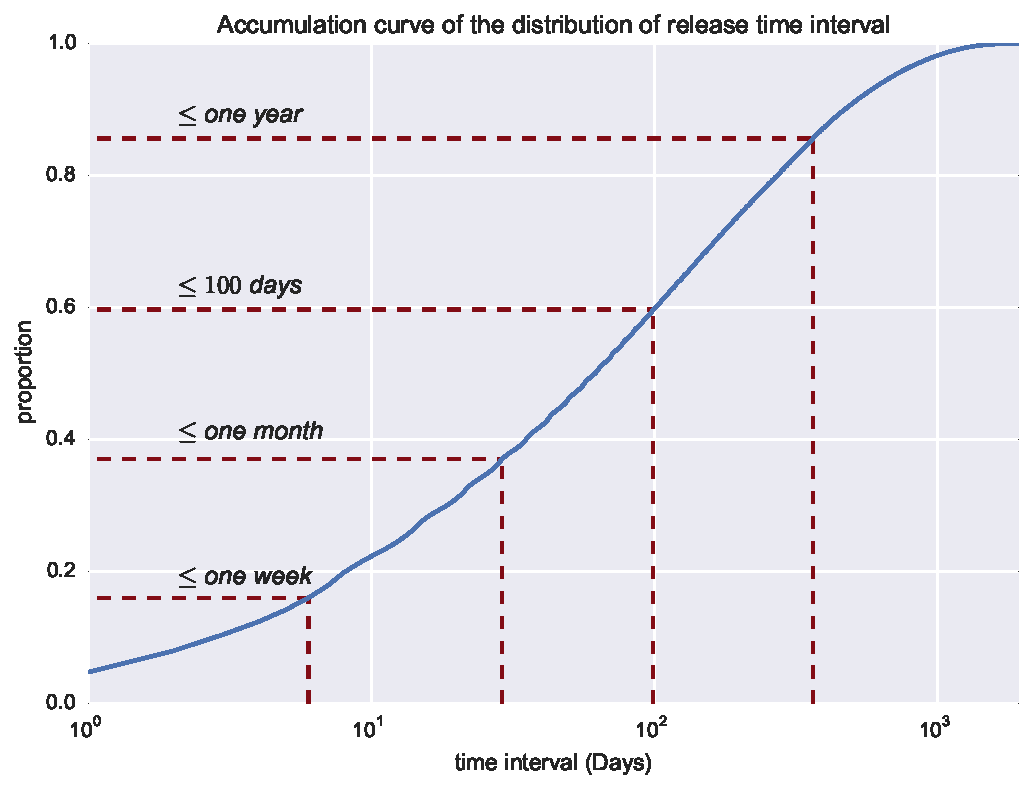
\includegraphics[width=0.8\textwidth]{fig/release_related}
    \caption{}
    \label{fig:release_relate}
\end{figure}

\subsection{Feature Generation}
\label{sec:6.2}

Each feature is computed from the comparison of two articles in a specific field. The value range of each feature is normalized to $0 \sim 1$. One type of features is the semantic textual similarity over particular text fields, such as \tfidf{} similarity and LSI similarity. Another type is the comparison of meta-data between articles. The computation of remaining features is defined as follows.
\begin{description}
    \item[\texttt{category}] This feature indicates the category relevance between two articles. Each article belongs to a category. Let $d_i$ denote the $i$-th article and $c_i$ denote the category of the $i$-th article. Each related article-pair $\langle d_i, d_j \rangle$ has a corresponding category-pair $\langle c_i, c_j \rangle$. The number of category is marked as $n$. After group all category-pairs, we obtain the $n \times n$ matrix $\mathbf{M}$, where $\mathbf{M}_{ij}$ refers to the probability of an article from category $i$ being related to articles from category $j$. Hence, feature \texttt{category} of an article-pair $\langle d_i, d_j \rangle$ is $\mathbf{M}_{c_i,c_j}$.

    \item[\texttt{keyword}] This feature indicates the keyword relevance between two articles. First, the inverse-document-frequency (\textit{idf}) of each keyword is computed with $$idf_k=log_2 \dfrac{\text{number of all articles}}{\text{number of articles containing keyword}~~k}$$, where $k$ is a keyword. Assuming a series of keywords $\mathbf{K}={k_1, \cdots, k_m}$ which occur in both of two articles $d_i$ and $d_j$, we compute feature \texttt{keyword} with $\sum_{i=1}^{m} idf_{k_i}$. The normalization of the feature is to divide each score by the greatest score for a particular target article. 
        
    \item[\texttt{release time}] This feature indicates the relevance of issue time between two articles. Let $r_i$ denote the release time of the corresponding article $d_i$. The time interval is computed with $\Delta_{ij}=|r_i - r_j|$. \\ After normalizing, feature $\mathtt{release~time} = \begin{cases} \dfrac{\Delta_{ij}}{\text{one year}} & \Delta_{ij} < \text{one year} \\ 1& \Delta_{ij} \ge \text{one year} \end{cases}$.
    
    \item[\texttt{number of terms}] This feature indicates the used-term relevance between two articles. For each article-pair, feature \texttt{number of terms} is the ratio of the smaller number of used terms of one article to the larger number of used term of another article over text field \icontent{}. 
    
    \item[\texttt{number of words}] This feature indicates the length relevance between two articles. For each article-pair, feature \texttt{number of words} is the ratio of the number of tokens of the shorter article to the number of tokens of the longer article. 
\end{description}

Now we have $3$ features including \texttt{category}, \texttt{keyword} and \texttt{release time} which are generated from the ``meta-data'', $2$ features including \texttt{number of terms} and \texttt{number of words} which are ``extracted'' from the \icontent{}, and $11$ STS features which are determined in table \ref{tab:select}. In order to describe the STS features simply, each such feature is denoted by a short symbol. The symbol is in the format of \texttt{\{n\}\{f\}-\{m\}}, where \texttt{\{n\}} denotes an n-gram model and the possible values are $1$, $2$ and $3$, \texttt{\{f\}} denotes a text field, and \texttt{\{m\}} denotes a STS method. In terms of \texttt{\{f\}}, the possible assignments are \textit{c}, \textit{t} and \textit{s}, which refer to \icontent{}, \ititle{} and \isummary{}, respectively. In respect of \texttt{\{m\}}, \textit{j}, \textit{t} and \textit{l} denote method Jaccard, \tfidf{} and LSI, respectively. For example, ``1c-t'' means method \tfidf{} for the unigram over \icontent{}.


\subsection{Supervised Methods}
\label{sec:6.3}

\subsection{Experimental Results}
\label{sec:6.4}

\begin{table}[]
\centering
\begin{tabular}{llrrr}
\textbf{No.} & \textbf{Combination of Features} & \textbf{LogReg} & \textbf{MART} & \textbf{ListNet} \\ \hline
\#00 & 1c-t (BASLINE) & 0.451 & 0.451 & 0.451 \\ \hline
\#01 & 1c-t, 1c-l & 0.458 & 0.445 & 0.453 \\
\#02 & 1c-t, 1c-l, 1t-t, 1s-t & 0.468 & 0.473 & 0.465 \\
\#03 & 1c-t, 1c-l, 2c-t, 3c-j & 0.485 & 0.464 & 0.481 \\
\#04 & all selected STS methods over text fields & 0.489 & 0.487 & 0.493 \\
\#05 & category + \#01 & 0.467 & 0.445 & 0.460 \\
\#06 & category + \#02 & 0.470 & 0.471 & 0.432 \\
\#07 & category + \#04 & 0.492 & 0.487 & 0.460 \\
\#08 & keyword + \#01 & 0.475 & 0.464 & 0.482 \\
\#09 & keyword + \#02 & 0.494 & 0.476 & 0.480 \\
\#10 & keyword + \#04 & 0.508 & 0.490 & 0.495 \\
\#11 & release + \#01 & 0.617 & 0.590 & 0.628 \\
\#12 & release + \#02 & 0.623 & 0.609 & 0.615 \\
\#13 & release + \#04 & 0.630 & \textbf{0.622} & 0.588 \\
\#14 & meta-data + \#01 & 0.629 & 0.593 & 0.598 \\
\#15 & meta-data + \#02 & \textbf{0.640} & 0.599 & \textbf{0.637} \\
\#16 & meta-data + \#04 & 0.635 & 0.619 & 0.633 \\
\#17 & meta-data + extend-data + \#01 & 0.628 & 0.587 & 0.605 \\
\#18 & meta-data + extend-data + \#02 & \textbf{0.640} & 0.605 & 0.608 \\
\#19 & meta-data + extend-data + \#04 & 0.634 & 0.612 & 0.585 \\ \hline
\end{tabular}
\caption{My caption}
\label{my-label}
\end{table}

如何计算最终的precision
对一个testing target,对每一篇在corpus中的文章生成一条数据,经过regressor之后得到一个probability of related article,然后选取概率最大的两条数据对应的文章作为最终的related articles. 然后计算平局precision与上个section方法一样。

在实验中,采用了几种可以regression的方法,分别为logistic regression, Bayesian regression 和XX。 

给出不同组合的结论得到最好的组合,并将最优模型带入实验二中,检测在reality中的实验结果是否一致。 
